\documentclass[UTF8,12pt]{article}
\usepackage{ctex}
\usepackage{indentfirst}
\usepackage{color}
\usepackage{hyperref}
\usepackage{graphicx}
\usepackage{subfigure}
\usepackage{pdfpages}
\usepackage{listings}
\usepackage{afterpage}
\usepackage{geometry}
\usepackage{booktabs}
\usepackage{multirow}
\usepackage{graphicx}

\geometry{a4paper,scale=0.8}

\newcommand\myemptypage{
    \null
    \thispagestyle{empty}
    \addtocounter{page}{-1}
    \newpage
}

\hypersetup{
    hidelinks,
	colorlinks=true,
	allcolors=black,
	pdfstartview=Fit,
	breaklinks=true
}

\definecolor{dkgreen}{rgb}{0,0.6,0}
\definecolor{gray}{rgb}{0.5,0.5,0.5}
\definecolor{mauve}{rgb}{0.58,0,0.82}

\lstset{ %
  language=Octave,                % the language of the code
  basicstyle=\footnotesize,           % the size of the fonts that are used for the code
  numbers=left,                   % where to put the line-numbers
  numberstyle=\tiny\color{gray},  % the style that is used for the line-numbers
  stepnumber=2,                   % the step between two line-numbers. If it's 1, each line 
                                  % will be numbered
  numbersep=5pt,                  % how far the line-numbers are from the code
  backgroundcolor=\color{white},      % choose the background color. You must add \usepackage{color}
  showspaces=false,               % show spaces adding particular underscores
  showstringspaces=false,         % underline spaces within strings
  showtabs=false,                 % show tabs within strings adding particular underscores
  frame=single,                   % adds a frame around the code
  rulecolor=\color{black},        % if not set, the frame-color may be changed on line-breaks within not-black text (e.g. commens (green here))
  tabsize=2,                      % sets default tabsize to 2 spaces
  captionpos=b,                   % sets the caption-position to bottom
  breaklines=true,                % sets automatic line breaking
  breakatwhitespace=false,        % sets if automatic breaks should only happen at whitespace
  title=\lstname,                   % show the filename of files included with \lstinputlisting;
                                  % also try caption instead of title
  keywordstyle=\color{blue},          % keyword style
  commentstyle=\color{dkgreen},       % comment style
  stringstyle=\color{mauve},         % string literal style
  escapeinside={\%*}{*)},            % if you want to add LaTeX within your code
  morekeywords={*,...}               % if you want to add more keywords to the set
}


\setlength{\parindent}{2em}

\begin{document}

\begin{titlepage}
    \includepdf[pages={1}]{cover.pdf}
\end{titlepage}

\myemptypage

\begin{center}
    \tableofcontents
\end{center}

\newpage

\section{实验1《GPIO端口实验》}

实验学时:2

每组人数:3

实验类别:2\ (1:基础性\ 2:综合性\ 3:设计性\ 4:研究性)

实验要求:1\ (1:必修\ 2:选修\ 3:其它)

实验类别:3\ (1:基础\ 2:专业基础\ 3:专业\ 4:其它)

\subsection{实验目的}
\begin{enumerate}
    \item 熟悉并掌握Keil MDK开发环境的使用以及在线调试方法;
    \item 掌握STM32F746NG芯片GPIO端口寄存器的配置;
    \item 通过实验掌握Cortex-M7控制GPIO端口的方法,实现对LED的控制。
\end{enumerate}

\subsection{实验内容}
编写程序,对指定GPIO端口进行初始化并完成配置过程,实现对LED的控制。学习使用超级终端,对其进行配置并完成串口调试。实验中观察GPIO端口输出数据寄存器(GPIOx\_ODR)的值对LED灯的明灭的影响,学习GPIO端口的输入输出方式、输出类型和输出速度的设置方法。

\subsection{实验方法}

\subsubsection{实验原理}
STM32F746NG芯片共有168个GPIO(通用I/O)端口(GPIOA~GPIOK),每个GPIO端口均可以通过软件配置为输出、输入或复用功能。

\begin{enumerate}
    \item GPIO主要特性
    \begin{itemize}
        \item 输出状态:推挽或开漏+上拉/下拉;
        \item 从输出数据寄存器(GPIOx\_ODR)或外设(复用功能输出)输出数据;
        \item 可为每个I/O选择不同的速度;
        \item 输入状态:浮空、上拉/下拉、模拟;
        \item 将数据输入到输入数据寄存器(GPIOx\_ODR)或外设(复用功能输入);
        \item 置位和复位寄存器(GPIOx\_BSRR),对GPIOx\_ODR具有按位写权限;
        \item 锁定机制(GPIOx\_LCKR),可冻结I/O端口配置;
        \item 模拟功能;
        \item 复用功能选择寄存器;
        \item 快速翻转,每次翻转最快只需要两个时钟周期;
        \item 引脚复用非常灵活,允许将I/O引脚用作GPIO或多种外设功能中的一种。
    \end{itemize}
    \item GPIO功能描述

    每个GPIO端口的各个端口位均可以自由编程,通过对相关寄存器的修改可以配置为多种模式:
    \begin{itemize}
        \item 浮空输入
        \item 上拉输入
        \item 下拉输入
        \item 模拟输入/输出
        \item 具有上拉或下拉功能的开漏输出
        \item 具有上拉或下拉功能的推挽输出
        \item 具有上拉或下拉功能的复用功能推挽
        \item 具有上拉或下拉功能的复用功能开漏
    \end{itemize}
    对I/O端口进行编程作为输入时,输出缓冲器被禁止,施密特触发器输入被打开,根据GPIOx\_PUPDR寄存器中的值决定是否打开上拉和下拉电阻,输入数据寄存器每隔1个AHB时钟周期对I/O引脚上的数据进行一次采样,对输入数据寄存器的读访问可获取I/O状态。

    对I/O端口进行编程作为输出时,输出缓冲器被打开,施密特触发器输入被打开,根据GPIOx\_PUPDR寄存器中的值决定是否打开上拉和下拉电阻,输入数据寄存器每隔1个AHB时钟周期对I/O引脚上的数据进行一次采样,对输入数据寄存器的读访问可获取I/O状态,对输出数据寄存器的读访问可获取最后的写入值。

    对I/O端口进行编程作为复用功能时,可将输出缓冲器配置为开漏或推挽模式,输出缓冲器由来自外设的信号驱动,施密特触发器输入被打开,根据GPIOx\_PUPDR寄存器中的值决定是否打开上拉和下拉电阻,输入数据寄存器每隔1个AHB时钟周期对I/O引脚上的数据进行一次采样,对输入数据寄存器的读访问可获取I/O状态。

    对I/O端口进行编程作为模拟配置时,输出缓冲器被禁止,施密特触发器输入停用,I/O引脚的每个模拟输入的功耗变为零,施密特触发器的输出被强制处理为恒定值(0),弱上拉和下拉电阻被硬件关闭,对输入数据寄存器的读访问值为“0”。

    \item GPIO寄存器

    每个通用I/O端口包括4个32位配置寄存器(GPIOx\_MODER、GPIOx\_OTYPER、GPIOx\_OSPEEDR 和 GPIOx\_PUPDR)、2个32位数据寄存器(GPIOx\_IDR 和 GPIOx\_ODR)和1个32位置位/复位寄存器 (GPIOx\_BSRR)。此外,所有GPIO都包括1个32位锁定寄存器 (GPIOx\_LCKR) 和2个32位复用功能选择寄存器(GPIOx\_AFRH 和 GPIOx\_AFRL)。I/O端口寄存器必须按32位字、半字或字节进行访问。
    \item GPIO寄存器边界地址
    
    STM43F746NG的GPIO寄存器边界地址如表所示
    \begin{table}[!ht]
        \centering
        \begin{tabular}{|l|l|}
        \hline
            外设 & 寄存器边界地址  \\ \hline
            GPIOA & 0x4002 0000 – 0x4002 03FF  \\ \hline
            GPIOB & 0x4002 0400 – 0x4002 07FF  \\ \hline
            GPIOC & 0x4002 0800 – 0x4002 0BFF  \\ \hline
            GPIOD & 0x4002 0C00 – 0x4002 0FFF  \\ \hline
            GPIOE & 0x4002 1000 – 0x4002 13FF  \\ \hline
            GPIOF & 0x4002 1400 – 0x4002 17FF  \\ \hline
            GPIOG & 0x4002 1800 – 0x4002 1BFF  \\ \hline
            GPIOH & 0x4002 1C00 – 0x4002 1FFF  \\ \hline
            GPIOI & 0x4002 2000 – 0x4002 23FF  \\ \hline
        \end{tabular}
    \end{table}

    \item 实验电路
    
    实验电路如图所示

    \begin{figure}[htbp]
        \centering
        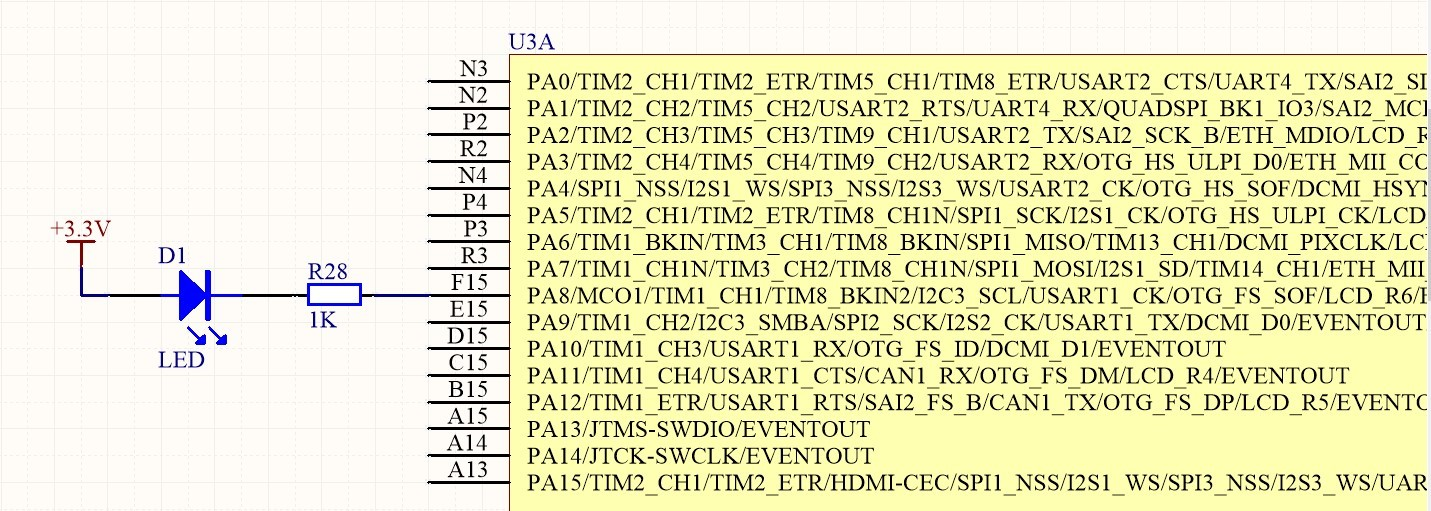
\includegraphics[width=0.8\textwidth]{imgs/1.jpg}
        \caption{实验电路}
    \end{figure}

    如图中所示,U3A单元为STM32F746芯片,发光二极管D1一端与VCC相连,另一端经过1K电阻与Cortex-M7的PA8(GPIOA8)相连,将PA8配置为输出I/O口,即可通过控制其高低电平状态进而控制发光二极管D1的的亮与灭。当PA8输出低电平时,电路导通,发光二极管D1点亮;反之,发光二极管D1熄灭。实验例程中,每次对PA8的输出状态取反后调用延时函数,使发光二极管保持亮或灭,循环往复即可实现发光二极管的闪烁。通过修改延时长度,可以改变发光二极管的闪烁频率。

\end{enumerate}

\subsubsection{实验方案及调试过程}
\noindent
\textbf{基础实验}:首先复现例程代码,得到指导书期望现象并记录
\noindent
实验例程如下:

\begin{lstlisting}[frame=shadowbox]
    /**
    主程序:系统上电初始化后对GPIO中的PA8进行配置,将其配置为输出端口并控制LED闪烁。
  **/
  #include "main.h"
  #include "system_init.h"
  
  /* Private variables */
  uint16_t delay = 100;
  
  void System_Init(void);
  void GPIO_Config(void);
  
  /* main */
  int main(void)
  {
    System_Init();
    
    GPIO_Config();
    
    printf("\n\rExample finished\n\r");
      
    /* Toggle IOs in an infinite loop */
    while (1)
    {
      HAL_GPIO_TogglePin(GPIOA, GPIO_PIN_8);
      /* Insert delay */
      HAL_Delay(delay);
    }
  }  
\end{lstlisting}
调试过程如下:

首先定义了私有变量delay,用于控制延时时间:uint16\_t delay = 100;

然后调用System\_Init()函数进行系统初始化,调用GPIO\_Config()函数对GPIO端口进行初始化。

\begin{lstlisting}[frame=shadowbox]
void System_Init(void)
{
  /* Enable the CPU Cache */
  CPU_CACHE_Enable();

  /* STM32F7xx HAL library initialization */
  HAL_Init();

  /* Configure the system clock to 216 MHz */
  SystemClock_Config();
  
  /* Configure UART */
  UART_Config();
  
  printf("\n\rSystem initialize success\n\r");
}
\end{lstlisting}
GPIO\_Config()函数的定义如下:

\begin{lstlisting}[frame=shadowbox]
void GPIO_Config(void)
{
/* Enable each GPIO Clock (to be able to program the configuration registers) */
  __HAL_RCC_GPIOA_CLK_ENABLE();
  
  /* Configure IOs in output push-pull mode to drive external LED */
  GPIO_InitStruct.Mode  = GPIO_MODE_OUTPUT_PP;	// 推挽输出
  GPIO_InitStruct.Pull  = GPIO_PULLUP;					// 上拉
  GPIO_InitStruct.Speed = GPIO_SPEED_HIGH;			// 高速

  GPIO_InitStruct.Pin = GPIO_PIN_8;
  HAL_GPIO_Init(GPIOA, &GPIO_InitStruct);				// 引脚为PA8
}

\end{lstlisting}
然后进入死循环状态,通过调用HAL\_GPIO\_TogglePin()函数对GPIOA的8号引脚进行翻转,即实现LED灯的闪烁效果。具体的实现如下:

\begin{lstlisting}[frame=shadowbox]
void HAL_GPIO_TogglePin(GPIO_TypeDef* GPIOx, uint16_t GPIO_Pin)
{
  /* Check the parameters */
  assert_param(IS_GPIO_PIN(GPIO_Pin));

  GPIOx->ODR ^= GPIO_Pin;
}
\end{lstlisting}
利用异或操作实现对GPIO引脚状态的翻转。

每次翻转后调用HAL\_Delay()函数进行延时,延时时间为delay,以控制LED灯的闪烁频率。具体实现如下:

\begin{lstlisting}[frame=shadowbox]
__weak void HAL_Delay(__IO uint32_t Delay)
{
  uint32_t tickstart = 0;
  tickstart = HAL_GetTick();
  while((HAL_GetTick() - tickstart) < Delay)
  {
  }
}
\end{lstlisting}
HAL\_Delay()函数通过调用HAL\_GetTick()函数获取当前的系统滴答计数值,然后通过循环判断当前的系统滴答计数值与tickstart的差值是否小于Delay,若小于则继续循环,否则退出循环,从而实现延时效果。

\noindent
\textbf{进阶实验}:请自行搜索摩尔斯密码表,通过控制D1的亮灭间隔,实现自己姓氏拼音的电码实现。

摩尔斯电码(Morse code)也被称作摩斯密码,是一种时通时断的信号代码,通过不同的排列顺序来表达不同的英文字母、数字和标点符号。这里我们通过控制D1的亮灭间隔,实现自己姓氏拼音的电码。

具体的算法思路如下:

\begin{enumerate}
    \item 姓氏的拼音用英文打出,姓氏拼音有多个英文字母组成,英文字母之间用空格隔开,每一个姓之间用逗号隔开;
    \item 定义短信号和长信号的时间分别为200ms和600ms,空格时长1000ms,逗号时长2000ms,正常信号之间的间隔为200ms;
\end{enumerate}

第一步中,我们小组有三位成员,分别姓:
% // wjy-WU=".-- ..-"
% // gx-GUO="--. ..- ---"
% // zzy-ZOU="--.. --- ..-"

\begin{itemize}
    \item WU=".-- ..-"
    \item GUO="--. ..- ---"
    \item ZOU="--.. --- ..-"
\end{itemize}

因此我们定义字符数组:
\begin{lstlisting}[frame=shadowbox]
char lname[]=".-- ..-,--. ..- ---,--.. --- ..-";
\end{lstlisting}

然后定义短信号和长信号的时间分别为200ms和600ms,空格时长1000ms,逗号时长2000ms,正常信号之间的间隔为200ms。

\begin{lstlisting}[frame=shadowbox]
uint16_t delay = 100;
uint16_t short_delay=200;
uint16_t long_delay=600;
uint16_t blank_delay=1000;
uint16_t gap_delay=2000;
\end{lstlisting}

根据电码序列的不同字母('.'/'-'/' '/',')分别使用短延迟、长延迟、空格延迟、逗号延迟的时长进行延迟,从而控制灯亮灭的间隔。

在死循环中,对整个字符数组进行遍历,根据字符的不同,进行不同的延迟操作,从而实现对LED灯的控制。

\begin{lstlisting}[frame=shadowbox]
    while(1){
        //turn on the LED light
        HAL_GPIO_TogglePin(GPIOA, GPIO_PIN_8);
        if(lname[i%31]=='.'){
          HAL_Delay(short_delay);
        }else if(lname[i%31]=='-'){
          HAL_Delay(long_delay);
        }
        //turan off the LED light
        HAL_GPIO_TogglePin(GPIOA, GPIO_PIN_8);
        //control delay of off state
        if(lname[(i+1)%31]==' '){
          HAL_Delay(blank_delay);
          i+=2;
        }
        else if(lname[(i+1)%31]==','){
          HAL_Delay(gap_delay);
          i+=2;
        }else{
          HAL_Delay(delay);
          i++;
        }
    }
\end{lstlisting}

\subsection{实验步骤}
\subsubsection{准备实验环境}
使用ULINK2 USB-JTAG仿真器连接ARM Cortex-M7实验板与PC,实验板一侧接P1接口。使用串口线,连接实验板上的串口J3和PC机的串口。接口P1和J3的位置如图所示。

\begin{figure}[htbp]
    \centering
    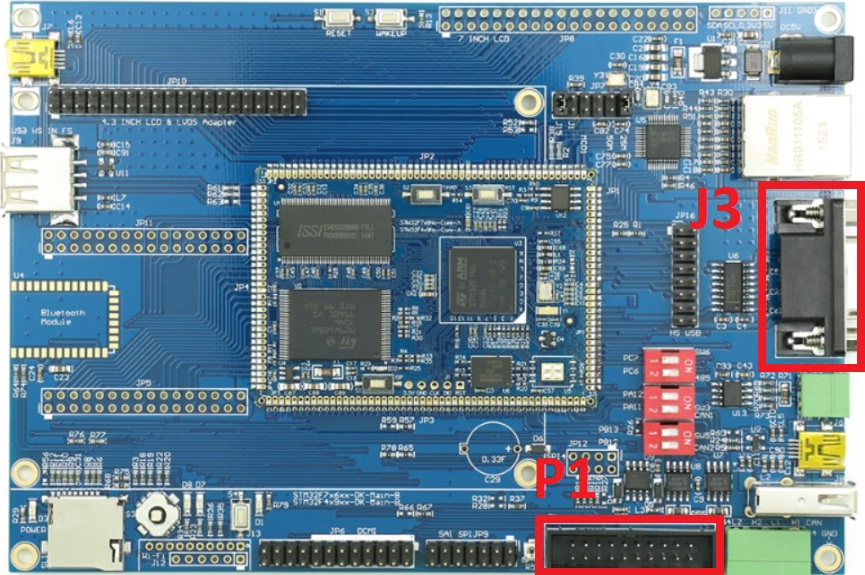
\includegraphics[width=0.8\textwidth]{imgs/2.png}
    \caption{接口P1和J3在实验板中的位置图}
\end{figure}

\subsubsection{串口接收设置}
在PC机上运行windows自带的超级终端串口通信程序(波特率115200 、1 位停止位、无校验位、无硬件流控制);或者使用其它串口通信程序。 

\subsubsection{打开实验例程}
拷贝实验平台附带程序“02\_GPIO”,使用$\mu$Vision IDE for ARM通过 ULINK2 USB-JTAG仿真器连接实验板,打开工程文件,编译链接工程,点击MDK的Project菜单,选择Rebuild all target files进行编译,编译成功后,点击Debug菜单,选择Start/Stop Debug Session项或点击工具栏中的 图标,下载工程生成的.axf 文件到目标板的 RAM中调试运行。

\subsubsection{观察实验结果}
结合实验内容和相关资料,使用一些调试命令,观察程序运行。注意观察发光二极管的亮灭情况,观察到的现象与前面实验内容中的相符,则说明实验程序通过配置GPIO引脚的输出状态实现了对发光二极管的控制。修改代码,实现自己姓氏的摩尔斯电码。

\subsection{实验结果}

\subsection{实验结论}
本实验中,我们通过HAL\_GPIO\_TogglePin()可以切换LED灯状态,利用异或(XOR)操作取反GPIOx对应位的值,达到反转指定引脚状态的效果;同时,我们可以通过控制HAL\_GPIO\_TogglePin()的间隔来控制亮灯和灭灯的时间,对不同的字符设置不同的间隔时间来实现自己姓氏拼音的电码。实验源代码见附录。

\subsection{实验小结}
通过本实验,我更加熟练地掌握了vscode+Keil MDK开发环境的使用以及在线调试方法,对STM32F746NG芯片GPIO端口寄存器的配置有了更加直观的认识,并对C语言嵌入式编程有了初步的认识,收获很大。

\newpage

% 一、实验目的
% 指出此次实验应该达到的学习目标。
% 二、实验内容
% 指出此次实验应完成的任务。
% 三、实验方法
% 包括实验方法、原理、技术、方案等。
% 四、实验步骤
% 指出完成该实验的操作步骤。
% 五、实验结果
% 记录实验输出数据和结果。
% 六、实验结论
% 对实验数据和结果进行分析描述,给出实验取得的成果和结论。
% 注:有程序的要求附上程序源代码,有图表的要有截图并有相应的文字说明和分析
% 七、实验小结
% 给出本次实验的体会,如学会了什么,遇到哪些问题,如何解决这些问题,存在哪些有待改进的地方。

\section{实验2《中断实验》}

实验学时:2

每组人数:3

实验类别:2\ (1:基础性\ 2:综合性\ 3:设计性\ 4:研究性)

实验要求:1\ (1:必修\ 2:选修\ 3:其它)

实验类别:3\ (1:基础\ 2:专业基础\ 3:专业\ 4:其它)

\subsection{实验目的}
\begin{itemize}
  \item 掌握外部中断的处理流程;
  \item 掌握Cortex-M7处理器的中断方式和中断处理过程;
  \item 通过实验学习Cortex-M7处理器的中断响应流程;
  \item 通过实验掌握Cortex-M7处理器中断处理的软件编程方法;
  \item 通过实验掌握Cortex-M7处理器中断响应过程中相关寄存器的使用方法。
\end{itemize}

\subsection{实验内容}
编写程序,对指定GPIO端口进行初始化,完成外部中断相关寄存器的配置,使用ARM Cortex-M7实验平台的按键S3产生外部中断,在中断响应过程中对LED进行控制,并采用不同的中断设置方法实现多种中断触发方式。实验过程中观察上升沿触发选择寄存器(EXTI\_RTSR)和下降沿触发选择寄存器(EXTI\_FTSR)的值对中断触发条件的影响,学习Cortex-M7外部中断线的设置方法和初始化,以及外部中断的触发方式和响应过程。

\subsection{实验方法}
\subsubsection{实验原理}
\begin{enumerate}
  \item STM32F746NG的外部中断和事件控制器(EXTI)
  
  STM32F746NG具有多达24个用于产生中断/事件请求的边沿检测器(输入线)。每根输入线都可以单独进行配置,以选择类型(中断或事件)和响应的触发事件(上升沿触发、下降沿触发或边沿触发),每根输入线还可以单独屏蔽。挂起寄存器用于保持中断请求。
  EXTI控制器的主要特性如下:
  \begin{itemize}
    \item 每个中断/事件线上都具有独立的触发和屏蔽;
    \item 每个中断线具有专用的状态位;
    \item 支持多大24个软件事件/中断请求;
    \item 检测脉冲宽度低于APB2时钟宽度的外部信号。
  \end{itemize}
  要产生中断,必须先配置好并使能中断线。根据需要的边沿检测设置2个触发寄存器,同时在中断屏蔽寄存器的相应位写“1”使能中断请求。当外部中断线上出现选定信号沿时,便会产生中断请求,对应的挂起位也会置1。在挂起寄存器的对应位写“1”,将清除该中断请求。
  要产生事件,必须先配置好并使能事件线。根据需要的边沿检测设置2个触发寄存器,同时在事件屏蔽寄存器的相应位写“1”使能事件请求。当事件线上出现选定信号沿时,便会产生事件脉冲,对应的挂起位会置1。
  通过在软件中对中断/事件寄存器写“1”,也可以产生中断/事件请求。
  要将一根输入线配置为中断源,需执行以下步骤:
  \begin{enumerate}
    \item 配置相应的屏蔽位(EXTI\_IMR);
    \item 配置中断线的触发选择位(EXTI\_RTSR和EXTI\_FTSR);
    \item 配置对应到外部中断控制器(EXTI)的NVIC中断通道的使能和屏蔽位,使得24个中断线中的请求可以被正确的响应。
  \end{enumerate}
  要将一根输入线配置为事件源,需执行以下步骤:
  \begin{enumerate}
    \item 配置相应的屏蔽位(EXTI\_EMR);
    \item 配置事件线的触发选择位(EXTI\_RTSR和EXTI\_FTSR);
  \end{enumerate}
  \item 外部中断/事件线映射及控制器框图
  
  如图所示,多达168个GPIO通过图中方式连接到16个外部中断/事件线。
  \begin{figure}[htbp]
    \centering
    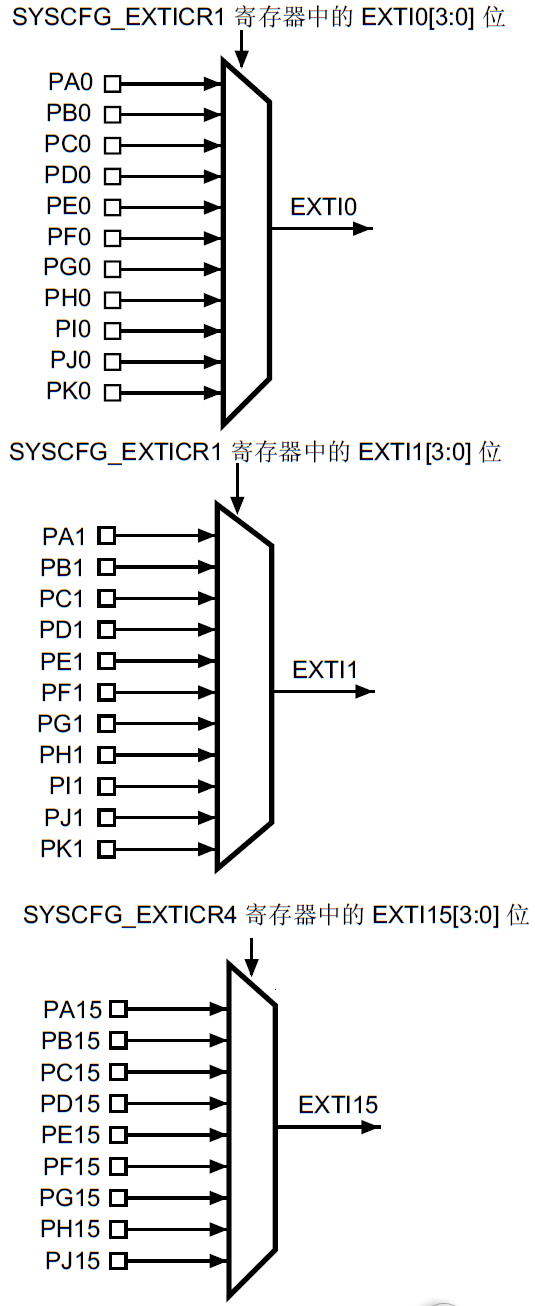
\includegraphics[width=0.3\textwidth]{imgs/3.png}
    \caption{外部中断/事件GPIO映射}
  \end{figure}
  另外8根EXTI线连接方式如下:
  \begin{itemize}
    \item EXTI16连接到PVD输出;
    \item EXTI17连接到RTC闹钟事件;
    \item EXTI18连接到USB OTG FS唤醒事件;
    \item EXTI19连接到以太网唤醒事件;
    \item EXTI20连接到USB OTG HS唤醒事件
    \item EXTI21连接到RTC侵入和时间戳事件
    \item EXTI22连接到RTC唤醒事件;
    \item EXTI23连接到LPTIM1异步事件。
  \end{itemize}
  EXTI控制器框图如图所示
  \begin{figure}[htbp]
    \centering
    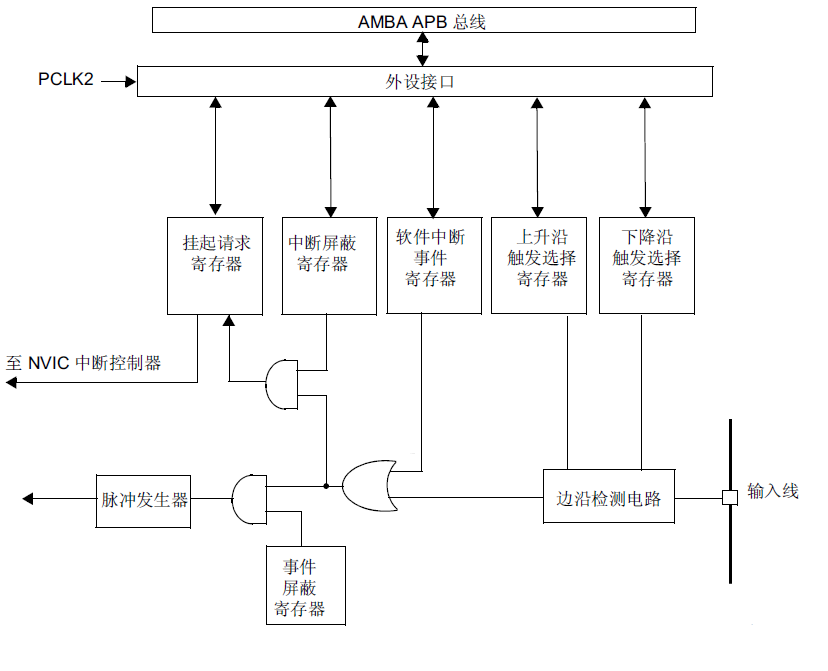
\includegraphics[width=0.3\textwidth]{imgs/4.png}
    \caption{EXTI控制器框图}
  \end{figure}

  \item EXTI寄存器
  
  \begin{enumerate}
    \item 中断屏蔽寄存器(EXTI\_IMR)
    
    偏移地址:0x00

    复位值:0x0000 0000

    中断屏蔽寄存器如图所示
    \begin{figure}[htbp]
      \centering
      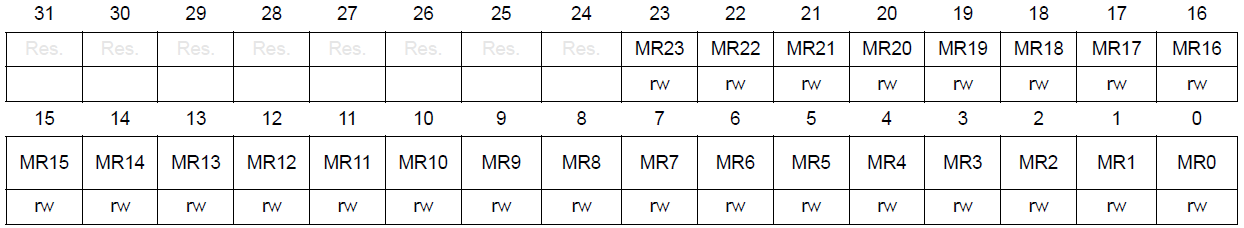
\includegraphics[width=0.8\textwidth]{imgs/5.png}
      \caption{中断屏蔽寄存器}
    \end{figure}

    位31:24保留,必须保持复位值。

    MRx:x线上的中断屏蔽

    0:屏蔽来自x线的中断请求

    1:开放来自x线的中断请求

    \item 事件屏蔽寄存器(EXTI\_EMR)
    
    偏移地址:0x04

    复位值:0x0000 0000

    事件屏蔽寄存器如图所示。

    \begin{figure}[htbp]
      \centering
      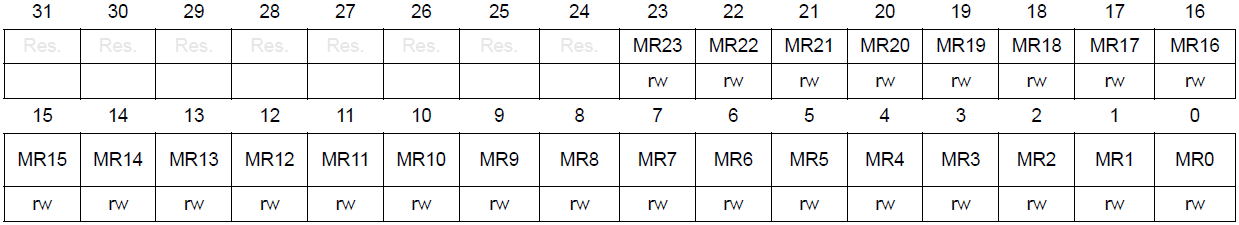
\includegraphics[width=0.8\textwidth]{imgs/6.png}
      \caption{事件屏蔽寄存器}
    \end{figure}

    位31:24保留,必须保持复位值。

    MRx:x线上的事件屏蔽

    0:屏蔽来自x线的事件请求

    1:开放来自x线的事件请求

    \item 上升沿触发选择寄存器(EXTI\_RTSR)
    
    偏移地址:0x08

    复位值:0x0000 0000

    上升沿触发选择寄存器如图所示。

    \begin{figure}[htbp]
      \centering
      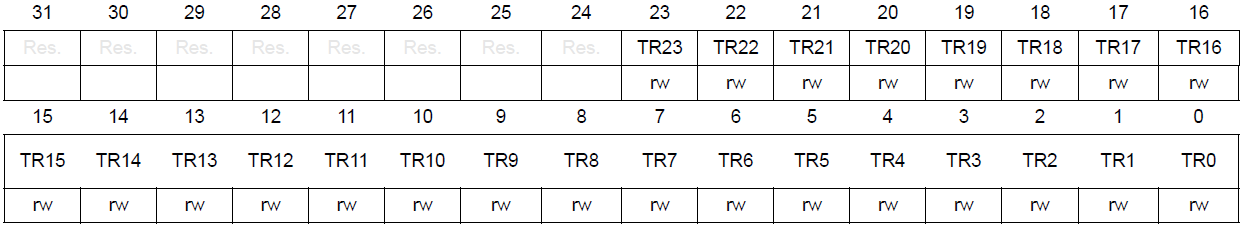
\includegraphics[width=0.8\textwidth]{imgs/7.png}
      \caption{上升沿触发选择寄存器}
    \end{figure}

    位31:24保留,必须保持复位值。

    TRx:x线的上升沿触发事件配置位

    0:禁止输入线上升沿触发(事件和中断)

    1:开放输入线上升沿触发(事件和中断)

    注:外部唤醒线配置为边沿触发时,在这些线上不能出现毛刺信号。
    
    如果在向EXTI\_RTSR寄存器写入值的同时外部中断线上产生上升沿,挂起位将被置位。
    
    在同一中断线上,可以同时设置上升沿和下降沿触发,即任一边沿都可触发中断。

    \item 下降沿触发选择寄存器(EXTI\_FTSR)
    
    偏移地址:0x0C

    复位值:0x0000 0000

    下降沿触发选择寄存器如图所示。

    \begin{figure}[htbp]
      \centering
      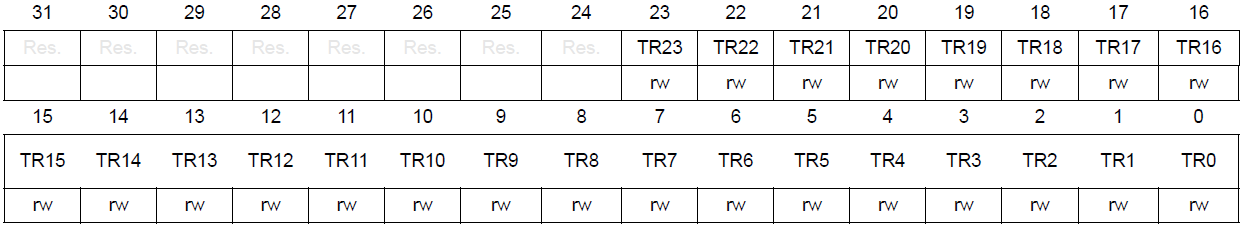
\includegraphics[width=0.8\textwidth]{imgs/8.png}
      \caption{下降沿触发选择寄存器}
    \end{figure}

    位31:24保留,必须保持复位值。

    TRx:x线的下降沿触发事件配置位

    0:禁止输入线下降沿触发(事件和中断)

    1:开放输入线下降沿触发(事件和中断)

    注:外部唤醒线配置为边沿触发时,在这些线上不能出现毛刺信号。

    如果在向EXTI\_FTSR寄存器写入值的同时外部中断线上产生下降沿,挂起位将被置位。

    在同一中断线上,可以同时设置上升沿和下降沿触发,即任一边沿都可触发中断。
    
    \item 软件中断事件寄存器(EXTI\_SWIER)
    
    偏移地址:0x10

    复位值:0x0000 0000

    软件中断事件寄存器如图所示。

    \begin{figure}[htbp]
      \centering
      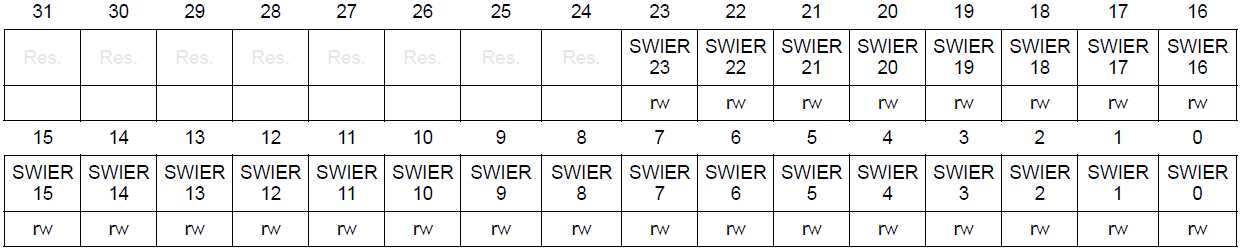
\includegraphics[width=0.8\textwidth]{imgs/9.png}
      \caption{软件中断事件寄存器}
    \end{figure}

    位31:24保留,必须保持复位值。

    SWIERx:x线的软件中断

    当SWIERx位设置为“0”时,将“1”写入该位会将EXTI\_PR寄存器中相应挂起位置1。如果在EXTI\_IMR寄存器中允许在x线上产生该中断,则产生中断请求。通过清除EXTI\_PR的对应位(写入“1”),可以清除该位为“0”。

    \item 挂起寄存器(EXTI\_PR)
    
    偏移地址:0x14

    复位值:未定义

    挂起寄存器如图所示。

    \begin{figure}[htbp]
      \centering
      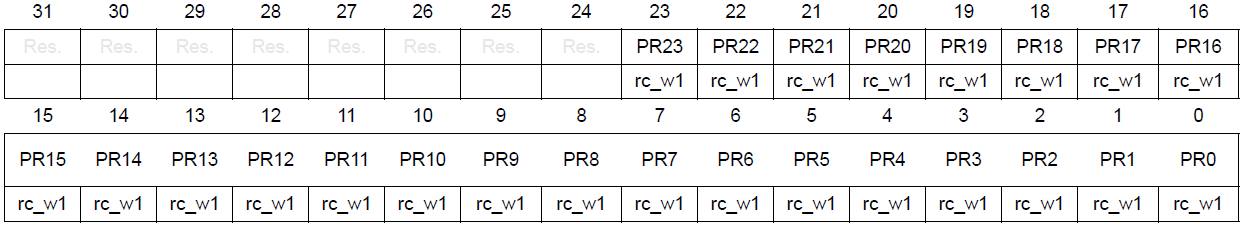
\includegraphics[width=0.8\textwidth]{imgs/10.png}
      \caption{挂起寄存器}
    \end{figure}

    位31:24保留,必须保持复位值。

    PRx:x线的挂起

    0:未发生触发请求

    1:发生了选择的触发请求

    注:当在外部中断线上发生了选择的边沿事件,该位被置1,将此位编程为“1”可清除此位。
  \end{enumerate}

  \item EXTI寄存器边界地址
  
  EXTI寄存器边界地为0x4001 3C00 – 0x4001 3FFF。

  \item 实验电路
  
  如图所示

  \begin{figure}[htbp]
    \centering
    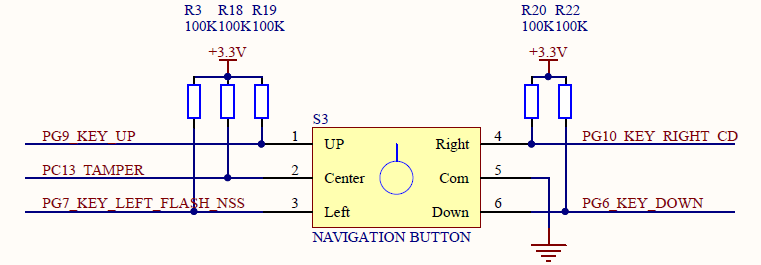
\includegraphics[width=0.8\textwidth]{imgs/11.png}
    \caption{实验电路}
  \end{figure}

  如图中所示,STM32F746芯片的PC13外接上拉电路,串联开关S3的Center(对应五向导航键S3的确定功能)后接地。由于I/O口外接上拉电路,所以在对I/O口进行初始化时可设置为浮空输入。开关S3断开时,PC13输入高电平;反之,PC13输入低电平。所以,当按下开关S3时,PC13输入由高变低,产生一个下降沿;当释放开关S3时,PC13输入由低变高,产生一个上升沿。根据外部中断触发条件设置,当满足所需的边沿条件时,触发中断,MCU响应中断点亮/熄灭发光二极管D1。
\end{enumerate}

\subsubsection{试验方案及调试过程}
\noindent
\textbf{基础实验}:本实验的实验例程(STM32F746\_Experiment\_v1.1/03\_EXTI)

实验例程如下:

\begin{lstlisting}[frame=shadowbox]
/**
  主程序:系统上电初始化后对LED1进行初始化,配置PC13作为外部中断源并开启中断,产生中断后点亮/熄灭LED。
**/
#include "main.h"
#include "system_init.h"

void System_Init(void);
void EXTI15_10_IRQHandler_Config(void);

/* main */
int main(void)
{
  System_Init();
  
  /* Initialize LED1 mounted on board */
  BSP_LED_Init(LED1);
  
  /* Configure EXTI15_10 (connected to PC.13 pin) in interrupt mode */
  EXTI15_10_IRQHandler_Config();
  
  while (1)
  {
  }
}

/* EXTI line detection callbacks, GPIO_Pin: Specifies the pins connected EXTI line */
void HAL_GPIO_EXTI_Callback(uint16_t GPIO_Pin)			//此处定义了HAL_GPIO_EXTI_Callback函数,原使用__weak  定义的函数被忽略�
{
  if (GPIO_Pin == GPIO_PIN_13)
  {
    /* Toggle LED1 */
    BSP_LED_Toggle(LED1);
    
    printf("\n\rLED1 switched\n\r");
  }
}
\end{lstlisting}
调试过程分析如下:

首先调用System\_Init()函数进行系统初始化,内部函数内容与实验一相同,不再赘述。

然后调用BSP\_LED\_Init()函数对LED1进行初始化,函数初始化板载LED1,使能LED1使其工作调用

\begin{lstlisting}[frame=shadowbox]
void BSP_LED_Init(Led_TypeDef Led)
{
  GPIO_InitTypeDef  gpio_init_structure;
  GPIO_TypeDef*     gpio_led;
	//Actualy only one LED
	switch(Led)
	{
		case LED1:
			/* Enable the GPIO_LED clock */
      LED1_GPIO_CLK_ENABLE();
			gpio_led = LED1_GPIO_PORT;
			break;
		case LED2:
			/* Enable the GPIO_LED clock */
      LED2_GPIO_CLK_ENABLE();
			gpio_led = LED2_GPIO_PORT;
			break;
		case LED3:
			/* Enable the GPIO_LED clock */
      LED3_GPIO_CLK_ENABLE();
			gpio_led = LED3_GPIO_PORT;
			break;
		case LED4:
			/* Enable the GPIO_LED clock */
      LED4_GPIO_CLK_ENABLE();
			gpio_led = LED4_GPIO_PORT;
			break;
		default:
			break;
	}
	/* Configure the GPIO_LED pin */
	gpio_init_structure.Pin = GPIO_PIN[Led];
	gpio_init_structure.Mode = GPIO_MODE_OUTPUT_PP;
	gpio_init_structure.Pull = GPIO_PULLUP;
	gpio_init_structure.Speed = GPIO_SPEED_HIGH;

	HAL_GPIO_Init(gpio_led, &gpio_init_structure);
	
	/* By default, turn off LED */
	HAL_GPIO_WritePin(gpio_led, GPIO_PIN[Led], GPIO_PIN_SET);
}
\end{lstlisting}
接着通过EXTI15\_10\_IRQHandler\_Config()函数配置PC13作为外部中断源并开启中断。

\begin{lstlisting}[frame=shadowbox]
void EXTI15_10_IRQHandler_Config(void)
{
  GPIO_InitTypeDef   GPIO_InitStructure;

  /* Enable GPIOC clock */
  __HAL_RCC_GPIOC_CLK_ENABLE();
	
  /* Configure PC.13 pin as input floating */
  GPIO_InitStructure.Mode = GPIO_MODE_IT_FALLING;				// 中断触发方式:下降沿触发
  GPIO_InitStructure.Pull = GPIO_NOPULL;								// GPIO内部无上拉或下拉
  GPIO_InitStructure.Pin = GPIO_PIN_13;
  HAL_GPIO_Init(GPIOC, &GPIO_InitStructure);						// 初始化PC13

  /* Enable and set EXTI lines 15 to 10 Interrupt to the lowest priority */
  HAL_NVIC_SetPriority(EXTI15_10_IRQn, 2, 0);						// 设置中断优先级
  HAL_NVIC_EnableIRQ(EXTI15_10_IRQn);										// 开中断
}
\end{lstlisting}
然后进入死循环,定义了下面的函数HAL\_GPIO\_EXTI\_Callback(),当发生中断时,自动调用该函数。该函数能够翻转LED1灯状态,从而完成改变LED灯亮灭状态的功能

\begin{lstlisting}[frame=shadowbox]
void HAL_GPIO_EXTI_Callback(uint16_t GPIO_Pin)			//此处定义了HAL_GPIO_EXTI_Callback函数,原使用__weak  定义的函数被忽略
{
  if (GPIO_Pin == GPIO_PIN_13)
  {
    /* Toggle LED1 */
    BSP_LED_Toggle(LED1);
    
    printf("\n\rLED1 switched\n\r");
  }
}
\end{lstlisting}

\noindent
\textbf{进阶实验}:按下按键触发中断LED灯高频闪烁,提起按键触发中断LED灯熄灭

具体的算法思路如下:

在config.c文件中配置中断触发方式为上升沿和下降沿(GPIO\_MODE\_IT\_RISING\_
FALLING),并设置一个全局变量down用来记录按键状态。HAL\_GPIO\_ReadPin () 可以读取按键状态,按下按键时为低电压,则为0,抬起按键时为高电压,即为1,实现的函数如下:

\begin{lstlisting}[frame=shadowbox]
void HAL_GPIO_EXTI_Callback(uint16_t GPIO_Pin){
  if(GPIO_Pin==GPIO_PIN_13){
    down=HAL_GPIO_ReadPin(GPIOC,GPIO_Pin);
  }
}
\end{lstlisting}
由此我们可以判断按键是否按键,并通过读取全局变量 down 值控制 LED 灯状态,实现按下按键时LED灯闪烁,松开按键时LED灯关闭。  

\begin{lstlisting}[frame=shadowbox]
int main(void)
{
  System_Init();
  
  /* Initialize LED1 mounted on board */
  BSP_LED_Init(LED1);
  
  /* Configure EXTI15_10 (connected to PC.13 pin) in interrupt mode */
  EXTI15_10_IRQHandler_Config();
  
  while (1)
  {
    if(down==0){
      BSP_LED_Toggle(LED1);
      HAL_Delay(short_delay);
      BSP_LED_Toggle(LED1);
      HAL_Delay(short_delay);
    }
  }
}
\end{lstlisting}

\subsection{实验步骤}

\subsubsection{准备实验环境}
使用ULINK2 USB-JTAG仿真器连接ARM Cortex-M7实验板与PC,实验板一侧接右下方的P1接口。使用串口线,连接实验板右侧的串口J3和PC机的串口。

\subsubsection{串口接收设置}
在PC机上运行windows自带的超级终端串口通信程序(波特率115200 、1 位停止位、无校验位、无硬件流控制);或者使用其它串口通信程序。

\subsubsection{打开实验例程}
拷贝实验平台附带程序“03\_EXTI”,使用$\mu$Vision IDE for ARM通过 ULINK2 USB-JTAG仿真器连接实验板,打开工程文件,编译链接工程,根据本实验指导书中2.3.2小节中“编译配置”部分对工程进行配置(工程默认已经配置正确),点击MDK的Project菜单,选择Rebuild all target files进行编译,编译成功后,点击Debug菜单,选择Start/Stop Debug Session项或点击工具栏中的 图标,下载工程生成的.axf 文件到目标板的 RAM中调试运行。

\subsubsection{观察实验结果}
结合实验内容和相关资料,使用一些调试命令,观察程序运行。注意观察按键S3按下和释放时发光二极管D1的亮灭情况,观察到的现象与前面实验内容中的相符,则说明实验程序通过将GPIO配置为EXTI的中断源,通过按键开关触发外部中断,MCU响应中断并点亮/熄灭发光二极管。修改部分代码,实现按下高频闪烁,松开熄灭的功能。

\subsection{实验结果}

\subsection{实验结论}
本实验中,我们首先观察到程序通过将GPIO配置为EXTI的中断源,通过按键开关触发外部中断,MCU响应中断并点亮/熄灭发光二极管。我们配置中断触发方式为上升沿和下降沿,并通过HAL\_GPIO\_ReadPin()读取按键状态,并根据按键状态控制 LED 灯状态,从而完成了实验要求的功能。实验源代码见附录。

\subsection{实验小结}
通过本实验,我更加熟练地掌握了Cortex-M7处理器的中断方式和中断处理过程,并熟悉了Cortex-M7处理器中断处理的软件编程方法和其中断响应过程中相关寄存器的使用方法,同时对嵌入式系统中电路与程序的关系有了进一步的认识,收获很大。

\newpage

\section{实验3《Uart+定时器实验》}

实验学时:2

每组人数:3

实验类别:2\ (1:基础性\ 2:综合性\ 3:设计性\ 4:研究性)

实验要求:1\ (1:必修\ 2:选修\ 3:其它)

实验类别:3\ (1:基础\ 2:专业基础\ 3:专业\ 4:其它)

\subsection{实验目的}

\subsection{实验内容}

\subsection{实验方法}

\subsection{实验步骤}

\subsection{实验结论}

\subsection{实验小结}

\newpage

\section{实验4《$\mu$C/OS-III 实验——信号量》}

实验学时:2

每组人数:3

实验类别:2\ (1:基础性\ 2:综合性\ 3:设计性\ 4:研究性)

实验要求:1\ (1:必修\ 2:选修\ 3:其它)

实验类别:3\ (1:基础\ 2:专业基础\ 3:专业\ 4:其它)

\subsection{实验目的}

\subsection{实验内容}

\subsection{实验方法}

\subsection{实验步骤}

\subsection{实验结论}

\subsection{实验小结}

\newpage

\section{附录}
\subsection{实验1源代码}
\begin{lstlisting}[frame=shadowbox]
    /**
    主程序:系统上电初始化后对GPIO中的PA8进行配置,将其配置为输出端口并控制LED闪烁。
  **/
  #include "main.h"
  #include "system_init.h"
  
  /* Private variables */
  uint16_t delay = 100;
  
  uint16_t short_delay=200;
  uint16_t long_delay=600;
  uint16_t blank_delay=1000;
  uint16_t gap_delay=2000;
  
  void System_Init(void);
  void GPIO_Config(void);
  
  /* main */
  int main(void)
  {
    System_Init();
    
    GPIO_Config();
    
    printf("\n\rExample finished\n\r");
  
    // wjy-WU=".-- ..-"
    // gx-GUO="--. ..- ---"
    // zzy-ZOU="--.. --- ..-"
    char lname[]=".-- ..-,--. ..- ---,--.. --- ..-";
    int i=0;
  
    /* Toggle IOs in an infinite loop */
    // while (1)
    // {
    //   HAL_GPIO_TogglePin(GPIOA, GPIO_PIN_8);
    //   /* Insert delay */
    //   HAL_Delay(delay);
    // }
  
    // 打印姓氏
    // 方法:
    // 形势的拼音用英文字母打出,每个字有多个英文字母组成,英文字母之间用空格隔开,每一个姓之间用逗号隔开
    // 设置长信号为600ms,短信号为200ms,空格为1000ms,姓之间间隔为2000ms,信号间隔100ms
    while(1){
      //turn on the LED light
      HAL_GPIO_TogglePin(GPIOA, GPIO_PIN_8);
      if(lname[i%31]=='.'){
        HAL_Delay(short_delay);
      }else if(lname[i%31]=='-'){
        HAL_Delay(long_delay);
      }
      //turan off the LED light
      HAL_GPIO_TogglePin(GPIOA, GPIO_PIN_8);
      //control delay of off state
      if(lname[(i+1)%31]==' '){
        HAL_Delay(blank_delay);
        i+=2;
      }
      else if(lname[(i+1)%31]==','){
        HAL_Delay(gap_delay);
        i+=2;
      }else{
        HAL_Delay(delay);
        i++;
      }
    }
  }  
\end{lstlisting}

\subsection{实验2源代码}
\begin{lstlisting}[frame=shadowbox]
/**
  主程序:系统上电初始化后对LED1进行初始化,配置PC13作为外部中断源并开启中断,产生中断后点亮/熄灭LED。
**/
#include "main.h"
#include "system_init.h"

void System_Init(void);
void EXTI15_10_IRQHandler_Config(void);

uint16_t short_delay=100;
uint16_t down=1;

/* main */
int main(void)
{
  System_Init();
  
  /* Initialize LED1 mounted on board */
  BSP_LED_Init(LED1);
  
  /* Configure EXTI15_10 (connected to PC.13 pin) in interrupt mode */
  EXTI15_10_IRQHandler_Config();
  
  while (1)
  {
    if(down==0){
      BSP_LED_Toggle(LED1);
      HAL_Delay(short_delay);
      BSP_LED_Toggle(LED1);
      HAL_Delay(short_delay);
    }
  }
}

/* EXTI line detection callbacks, GPIO_Pin: Specifies the pins connected EXTI line */
// void HAL_GPIO_EXTI_Callback(uint16_t GPIO_Pin)			//此处定义了HAL_GPIO_EXTI_Callback函数,原使用__weak  定义的函数被忽略
// {
//   if (GPIO_Pin == GPIO_PIN_13)
//   {
//     /* Toggle LED1 */
//     BSP_LED_Toggle(LED1);
    
//     printf("\n\rLED1 switched\n\r");
//   }
// }

void HAL_GPIO_EXTI_Callback(uint16_t GPIO_Pin){
  if(GPIO_Pin==GPIO_PIN_13){
    down=HAL_GPIO_ReadPin(GPIOC,GPIO_Pin);
  }
}
\end{lstlisting}

\subsection{实验3源代码}
\begin{lstlisting}[frame=shadowbox]
/**
  主程序:系统初始化后使用串口通信对Timer3的自动重载寄存器(ARR)初值进行选择,通过配置预分频,
	将Timer3的时钟频率设置为10KHz,在配置好定时器后开启定时器中断。Timer3的计数器寄存器从0开始以10KHz的频率递增,
	当其值大于ARR寄存器中的数值时,产生上溢,即定时器中断。
	注意:此例程中,每产生一次定时器中断,LED发生一次跳变,即模式1中LED闪烁频率为0.5Hz,模式2中LED闪烁频率为5Hz
**/
#include "main.h"
#include "system_init.h"

#define TIMEOUT   10000       // 10 seconds

/* Prescaler declaration */
uint8_t uRxBuffer = '1';			// 默认选择模式"1. 10000"
uint16_t ARRValue = 10000 - 1;// 默认ARR寄存器值为10000 - 1
extern UART_HandleTypeDef   UartHandle;
extern TIM_HandleTypeDef    TimHandle;

void System_Init(void);
void Timer_Config(uint16_t ARRValue);
    
/* main */
int main(void)
{
  System_Init();
  
  // printf("\n\r************************************\n\r");
  // printf("* Timer counter frequency is 10KHz *\n\r* Upcounting mode                  *\n\r* Initial value is 0               *");
  // printf("\n\r************************************\n\r");
  // printf("\n\rSelect the value of ARR register:\n\r1. 10000(default)    2. 1000\n\r");
  
  // /* Receive data from UART */
  // HAL_UART_Receive(&UartHandle, (uint8_t*)&uRxBuffer, 1, TIMEOUT);
  
  // if (uRxBuffer == '2')
  //   ARRValue = 1000 - 1;

  // Timer_Config(ARRValue);	//使用Tim3在这里面配置中断

  // /* Start the TIM Base generation in interrupt mode */
  // HAL_TIM_Base_Start_IT(&TimHandle);
  
  // printf("\n\rExample finished\n\r");
  
  while (1)
  {
    uint8_t stack[100];
    int store=0;

    double num=0;
    printf("\n\r**** UART-Timer ****\n\rPlease enter the frequency...\n\r");

    //receive data from uart
    while(1){
      HAL_UART_Receive(&UartHandle,(uint8_t*)&uRxBuffer,1,TIMEOUT);
      printf("%c",uRxBuffer);
      if(uRxBuffer!='\r'&&uRxBuffer!='\n'){
        if((uRxBuffer>='0'&&uRxBuffer<='9')||uRxBuffer=='.'){
          stack[store]=uRxBuffer;
          store++;
        }else{
          printf("\n\r INPUT ERROR! \n\r");
          break;
        }
      }

      if(uRxBuffer=='\r'||uRxBuffer=='\n'||store>10){
        sscanf((const char*)stack,"%lf",&num);
        ARRValue=5000/num-1;
        break;
      }
    }

    Timer_Config(ARRValue);

    HAL_TIM_Base_Start_IT(&TimHandle);
  }
}

void HAL_TIM_PeriodElapsedCallback(TIM_HandleTypeDef *htim)
{
  BSP_LED_Toggle(LED1);
}

\end{lstlisting}

\subsection{实验4源代码}
\begin{lstlisting}[frame=shadowbox]
/**
  主程序:上电后进行系统硬件初始化以及uC/OS-III初始化,完成初始化工作后创建启动
	任务:AppTaskStart,在该任务中完成板级支持包BSP和CPU模块的初始化,并创建
	两个应用任务Task_A和Task_B,其中Task_A检测按键S3是否被按下并释放,当S3释放时
	产生信号量,Task_B等待Task_A发送来的信号量,当获取到信号量时点亮/熄灭LED1并向
	串口发送数据。
**/
#include  <stdarg.h>
#include  <stdio.h>
#include  <math.h>
#include  <stm32f7xx_hal.h>
#include "stm32756g_eval.h"

#include  <cpu.h>
#include  <lib_math.h>
#include  <lib_mem.h>
#include  <os.h>
#include  <os_app_hooks.h>

#include  <app_cfg.h>
#include  <bsp.h>

#if (APP_CFG_SERIAL_EN == DEF_ENABLED)
#include  <app_serial.h>
#endif
/*
****************************************************
****************************************************
*
*                                            LOCAL DEFINES
****************************************************
****************************************************
*
*/

#define  APP_TASK_EQ_0_ITERATION_NBR              16u
#define  APP_TASK_EQ_1_ITERATION_NBR              18u


/*
****************************************************
****************************************************
*
*                                       LOCAL GLOBAL VARIABLES
****************************************************
****************************************************
*
*/
/* --------------- APPLICATION GLOBALS ---------------- */
static  OS_TCB       AppTaskStartTCB;
static  CPU_STK      AppTaskStartStk[APP_CFG_TASK_START_STK_SIZE];

/* --------------- SEMAPHORE TASK TEST --------------- */
static  OS_TCB       Task_ATCB;
static  CPU_STK      Task_AStk[APP_CFG_TASK_OBJ_STK_SIZE];

static  OS_TCB       Task_BTCB;
static  CPU_STK      Task_BStk[APP_CFG_TASK_OBJ_STK_SIZE];

#if (OS_CFG_SEM_EN > 0u)
static  OS_SEM       wait_key_sem;
static  OS_SEM       wait_key_sem2;
#endif

/*
****************************************************
****************************************************
*
*                                         FUNCTION PROTOTYPES
****************************************************
****************************************************
*
*/

static  void  AppTaskStart (void  *p_arg);
static  void  AppTaskCreate(void);
static  void  AppObjCreate (void);

static  void  Task_A(void *p_arg);
static  void  Task_B(void *p_arg);

/*
****************************************************
****************************************************
*
*                                                main()
*
* Description : This is the standard entry point for C code.  It is assumed that your code will call
*               main() once you have performed all necessary initialization.
*
* Arguments   : none
*
* Returns     : none
*
* Notes       : 1) STM32F7xx HAL library initialization:
*                      a) Configures the Flash prefetch, intruction and data caches.
*                      b) Configures the Systick to generate an interrupt. However, the function ,
*                         HAL_InitTick(), that initializes the Systick has been overwritten since Micrium's
*                         RTOS has its own Systick initialization and it is recommended to initialize the
*                         Systick after multitasking has started.
*
****************************************************
****************************************************
*
*/

int main(void)
{
    OS_ERR   err;
#if (CPU_CFG_NAME_EN == DEF_ENABLED)
    CPU_ERR  cpu_err;
#endif

    HAL_Init();                                                 /* 初始化HAL库                                          */

    Mem_Init();                                                 /* 初始化内存管理模块                                   */
    Math_Init();                                                /* 初始化数学算法模块(生成随机数种子)                 */

#if (CPU_CFG_NAME_EN == DEF_ENABLED)
    CPU_NameSet((CPU_CHAR *)"STM32F746xx",
                (CPU_ERR  *)&cpu_err);
#endif

    BSP_IntDisAll();                                            /* 关闭中断                                             */

    OSInit(&err);                                               /* 初始化uC/OS-III                                      */
    App_OS_SetAllHooks();

    OSTaskCreate(&AppTaskStartTCB,                              /* 创建启动进程                                         */
                  "App Task Start",
                  AppTaskStart,
                  0u,
                  APP_CFG_TASK_START_PRIO,
                 &AppTaskStartStk[0u],
                  AppTaskStartStk[APP_CFG_TASK_START_STK_SIZE / 10u],
                  APP_CFG_TASK_START_STK_SIZE,
                  0u,
                  0u,
                  0u,
                 (OS_OPT_TASK_STK_CHK | OS_OPT_TASK_STK_CLR),
                 &err);

    OSStart(&err);                                              /* 开启uC/OS-III                                        */

    while (DEF_ON) {                                            /* Should Never Get Here.                               */
        ;
    }
}


/*
****************************************************
****************************************************
*
*                                          STARTUP TASK
*
* Description : This is an example of a startup task.  As mentioned in the book's text, you MUST
*               initialize the ticker only once multitasking has started.
*
* Arguments   : p_arg   is the argument passed to 'AppTaskStart()' by 'OSTaskCreate()'.
*
* Returns     : none
*
* Notes       : 1) The first line of code is used to prevent a compiler warning because 'p_arg' is not
*                  used.  The compiler should not generate any code for this statement.
****************************************************
****************************************************
*
*/

static  void  AppTaskStart (void *p_arg)
{
    OS_ERR      err;
    CPU_INT32U  r0;
    CPU_INT32U  r1;
    CPU_INT32U  r2;
    CPU_INT32U  r3;
    CPU_INT32U  r4;
    CPU_INT32U  r5;
    CPU_INT32U  r6;
    CPU_INT32U  r7;
    CPU_INT32U  r8;
    CPU_INT32U  r9;
    CPU_INT32U  r10;
    CPU_INT32U  r11;
    CPU_INT32U  r12;


   (void)p_arg;

    r0  =  0u;                                                  /* Initialize local variables.                          */
    r1  =  1u;
    r2  =  2u;
    r3  =  3u;
    r4  =  4u;
    r5  =  5u;
    r6  =  6u;
    r7  =  7u;
    r8  =  8u;
    r9  =  9u;
    r10 = 10u;
    r11 = 11u;
    r12 = 12u;

    BSP_Init();                                                 /* 初始化板级支持包                                     */
    CPU_Init();                                                 /* 初始化CPU模块                                        */

#if OS_CFG_STAT_TASK_EN > 0u
    OSStatTaskCPUUsageInit(&err);                               /* Compute CPU capacity with no task running            */
#endif

#ifdef CPU_CFG_INT_DIS_MEAS_EN
    CPU_IntDisMeasMaxCurReset();
#endif

		UART_Config();
		
		/* Initialize LCD Communication for Application ...  		*/
		BSP_LCD_Config();
    APP_TRACE_DBG(("Creating Application kernel objects\r\n"));
		AppObjCreate();                                             /* 创建任务通信过程中使用的信号量等对象                 */

    APP_TRACE_DBG(("Creating Application Tasks\r\n"));
    AppTaskCreate();                                            /* 创建应用任务                                         */

    BSP_LED_Off(LED1);

    while (DEF_TRUE) {                                          /* 启动任务进入无限循环                                 */
        OSTimeDlyHMSM(0u, 0u, 0u, 100u,
                      OS_OPT_TIME_HMSM_STRICT,
                      &err);

        if ((r0  !=  0u) ||                                     /* Check task context.                                  */
            (r1  !=  1u) ||
            (r2  !=  2u) ||
            (r3  !=  3u) ||
            (r4  !=  4u) ||
            (r5  !=  5u) ||
            (r6  !=  6u) ||
            (r7  !=  7u) ||
            (r8  !=  8u) ||
            (r9  !=  9u) ||
            (r10 != 10u) ||
            (r11 != 11u) ||
            (r12 != 12u)) {
           APP_TRACE_INFO(("Context Error\r\n"));
        }
    }
}

/*
****************************************************
****************************************************
*
*                                          AppTaskCreate()
*
* Description : Create Application Tasks.
*
* Argument(s) : none
*
* Return(s)   : none
*
* Caller(s)   : AppTaskStart()
*
* Note(s)     : 该任务创建应用任务
****************************************************
****************************************************
*
*/

static  void  AppTaskCreate (void)
{
    OS_ERR  os_err;

/* ---------- 创建应用任务 --------- */
    OSTaskCreate(&Task_ATCB,
                 "Kernel Objects Task A",
                  Task_A,
                  0,
                  APP_CFG_TASK_OBJ_PRIO,
                 &Task_AStk[0],
                  Task_AStk[APP_CFG_TASK_OBJ_STK_SIZE / 10u],
                  APP_CFG_TASK_OBJ_STK_SIZE,
                  0u,
                  0u,
                  0,
                 (OS_OPT_TASK_STK_CHK | OS_OPT_TASK_STK_CLR),
                 &os_err);

    OSTaskCreate(&Task_BTCB,
                 "Kernel Objects Task B",
                  Task_B,
                  0,
                  APP_CFG_TASK_OBJ_PRIO,
                 &Task_BStk[0],
                  Task_BStk[APP_CFG_TASK_OBJ_STK_SIZE / 10u],
                  APP_CFG_TASK_OBJ_STK_SIZE,
                  0u,
                  0u,
                  0,
                 (OS_OPT_TASK_STK_CHK | OS_OPT_TASK_STK_CLR),
                 &os_err);
}

/*
****************************************************
****************************************************
*
*                                          AppObjCreate()
*
* Description : Create Application Kernel Objects.
*
* Argument(s) : none
*
* Return(s)   : none
*
* Caller(s)   : AppTaskStart()
*
* Note(s)     : 该任务创建任务通信过程中使用的信号量。
****************************************************
****************************************************
*
*/
static  void  AppObjCreate (void)
{
    OS_ERR  os_err;

#if (OS_CFG_SEM_EN > 0u)
    OSSemCreate(&wait_key_sem,
                "Key Detection",
                 0u,
                &os_err);
    OSSemCreate(&wait_key_sem2,"Key Detection",0u,&os_err);
#endif
}

/*
****************************************************
****************************************************
*
*                                          Task_A()
*
* Description : Test uC/OS-III objects.
*
* Argument(s) : p_arg is the argument passed to 'Task_A' by 'OSTaskCreate()'.
*
* Return(s)   : none
*
* Caller(s)   : This is a task
*
* Note(s)     : 该任务检测S3是否被按下并释放,当S3释放时向Task_B发送信号量。
****************************************************
****************************************************
*
*/
void Task_A(void *p_arg)
{	   
	OS_ERR  err;
	unsigned char key_press = 0;

	while(DEF_TRUE)
	{
	// 	OSTimeDly(30, OS_OPT_TIME_DLY, &err);
    // if (BSP_PB_GetState(BUTTON_TAMPER) == RESET)
	// 		key_press = 1;
	// 	if (BSP_PB_GetState(BUTTON_TAMPER) == SET)
	// 	{
	// 		if(key_press == 1)
	// 		{
	// 			key_press = 0;
	// 			OSSemPost(&wait_key_sem, OS_OPT_POST_1, &err);
	// 		}
	// 	}	
        OSTimeDly(60, OS_OPT_TIME_DLY, &err);
				if (BSP_PB_GetState(BUTTON_TAMPER) == RESET){
            OSSemPost(&wait_key_sem, OS_OPT_POST_1, &err);
        }
	}
}
/*
****************************************************
****************************************************
*
*                                          Task_B()
*
* Description : Test uC/OS-III objects.
*
* Argument(s) : p_arg is the argument passed to 'Task_B' by 'OSTaskCreate()'.
*
* Return(s)   : none
*
* Caller(s)   : This is a task
*
* Note(s)     : 该任务等待Task_A发送来的信号量,当获取到信号量时点亮/熄灭LED1并向串口发送数据。
****************************************************
****************************************************
*
*/
void Task_B(void *p_arg)
{			  
	OS_ERR  err;
	CPU_TS  ts;

	while(DEF_TRUE)
	{
		OSTimeDly(30, OS_OPT_TIME_DLY, &err);
		OSSemPend(&wait_key_sem,
                  0,
                  OS_OPT_PEND_BLOCKING,
                  &ts,
                  &err);
		BSP_LED_Toggle(LED1);	//Toggle after key release
        OSTimeDly(30, OS_OPT_TIME_DLY, &err);
        BSP_LED_Toggle(LED1);
		APP_TRACE_DBG(("Get a Semaphore from Task A\n\r"));
	}
}


\end{lstlisting}


\end{document}
